\chapter{Simulations of the Ground Level Enhancements for the Analysis of HiSPARC Station 14008}\label{app:GLE_sims}


\section{Model}

The artificial data used in the simulations of the \glspl{gle}, during the investigation of the performance of \gls{hisparc} station 14008, were created using a very simplistic model which was physically motivated by \gls{gle} observations \citep{strauss_pulse_2017}.

There were several variables that allowed us to change the physics of the simulations. These were:

\begin{itemize}
	%	\item{{\bf $N$}: Number of stations}
	\item{{\bf $T_d$}: Observing window}
	\item{{\bf $t_0$}: Time of \gls{gle} peak}
	\item{{\bf $\lambda$}}: Background count level
	\item{{\bf $\sigma$}}: Detector noise level
	\item{{\bf $A$}: Percentage amplitude of \gls{gle} increase}
	\item{{\bf $\tau_r$}: Rise time of \gls{gle}}
	\item{{\bf $\tau_d$}: Decay time of \gls{gle}}
\end{itemize}

Using these variables, the mathematical form of the model was expressed by:

\begin{equation}
    y(t) =  \sigma \, + \, \lambda \, (1 + A) \, . 
\begin{cases}

\exp\left[{\frac{t - t_0}{\tau_r}}\right] \,  & \text{if           $t \leq t_0$} \\

\exp\left[{-\frac{t - t_0}{\tau_d}}\right] \,  & \text{if           $t > t_0$} 

\end{cases} \, ,
\label{eq:GLE_model}
\end{equation}

where $t$ is the time in the range from 0 -- $T_d$ in 10-second intervals, to be representative of the real \gls{hisparc} station 14008 data.

An example time series of a single \gls{gle} is shown in Figure~\ref{fig:simulated_HS14008_GLE_data}. This shows both the model used to generate the simulated data (black line), as well as the background level and noise with and without the \gls{gle} injected, blue and orange lines, respectively.

\begin{figure}[ht!]
	\centering
	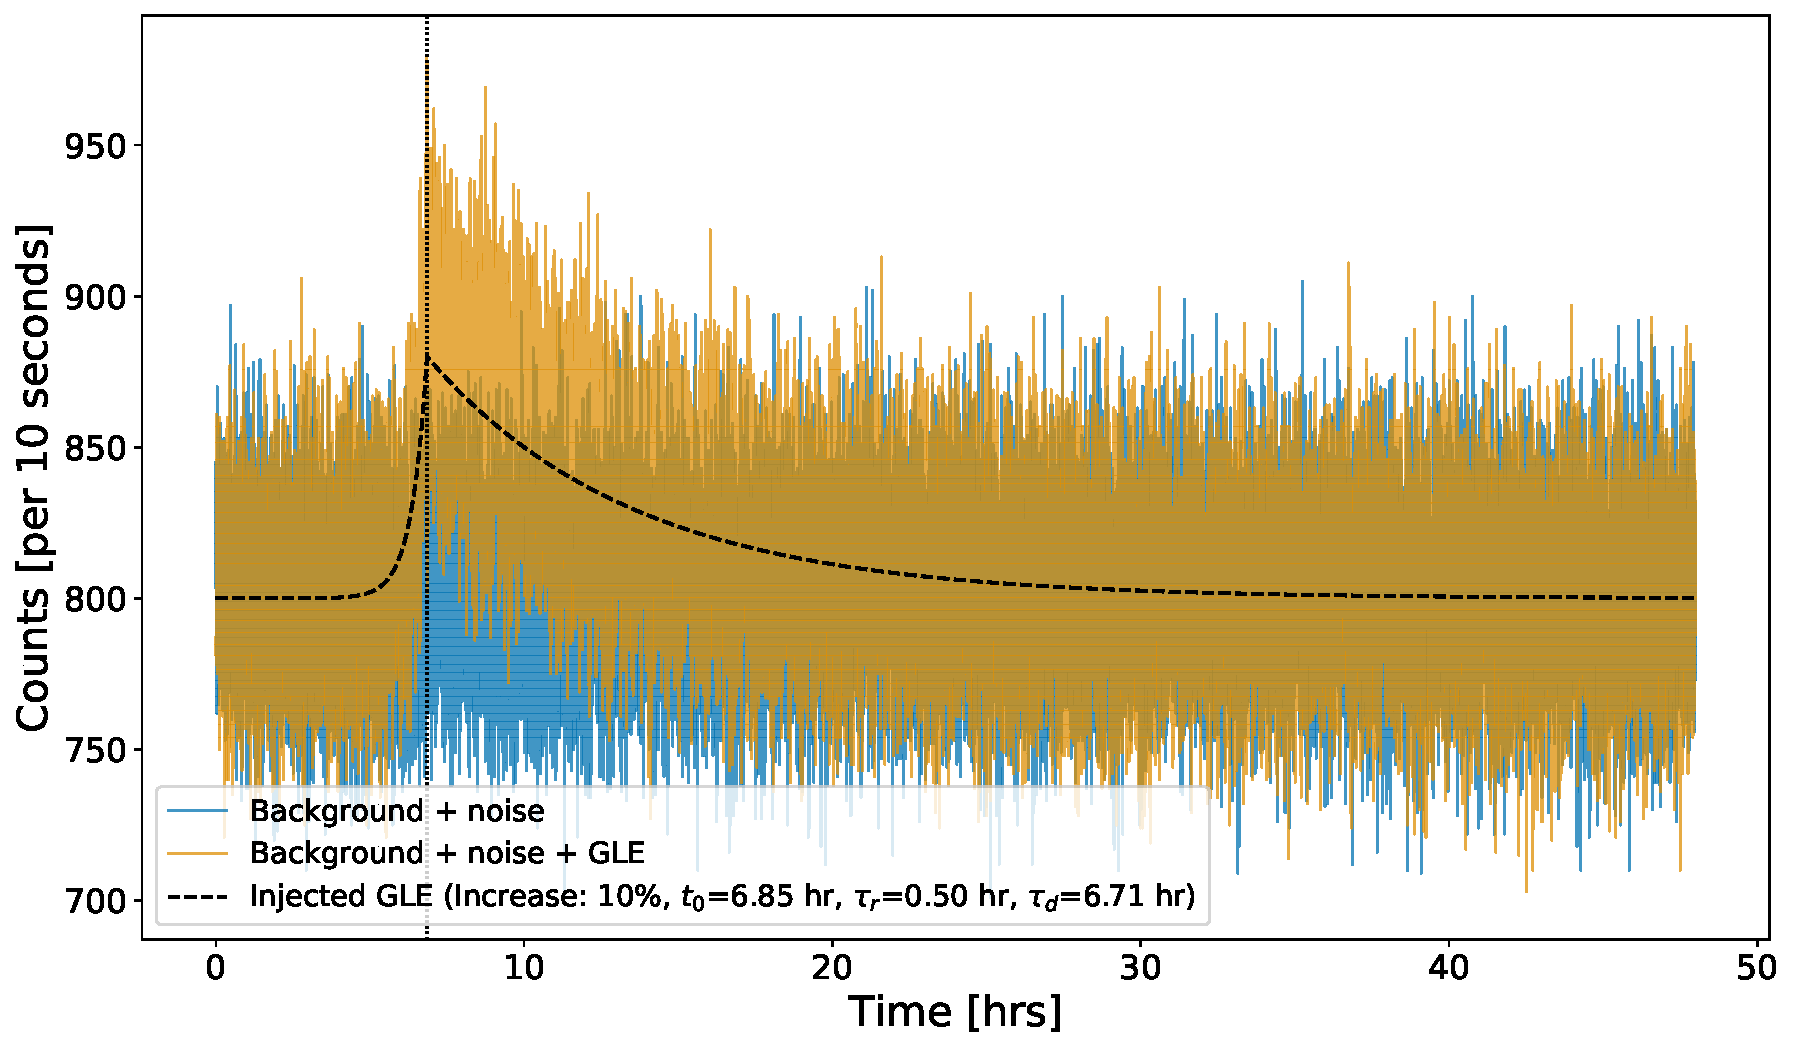
\includegraphics[width=\columnwidth]{simulated_HS14008_GLE_data.pdf}
	\caption{Example of a realisation of the simulations, to generate an artificial time series with a $10 \%$ GLE injected. The black line shows the model for the GLE. The blue line shows the realisation of the signal without a GLE injected, and the orange line shows the realisation of the model with the GLE injected.}
	\label{fig:simulated_HS14008_GLE_data}
\end{figure}


\section{Configuration of the Simulations}

The simulated data were generated using a Python script. A flowchart describing the steps in the simulation is shown in Figure~\ref{fig:gle_flowchart}. 

\begin{figure}[ht!]
	\centering
	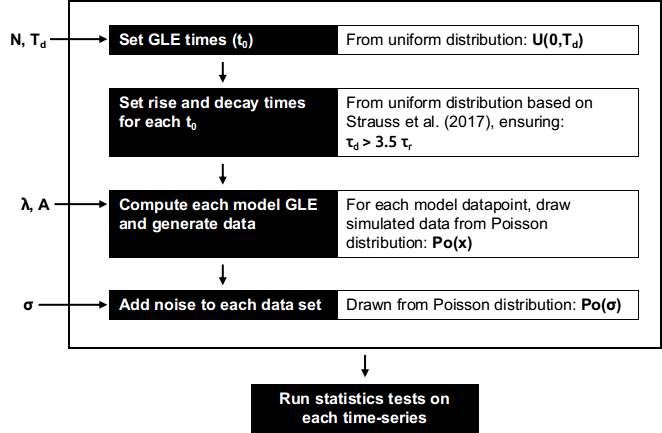
\includegraphics[width=0.9\columnwidth]{GLE_sims_flowchart.png}
	\caption{Flowchart showing the step-by-step processes in the generation of the artificial HiSPARC 14008 GLE time series data.}
	\label{fig:gle_flowchart}
\end{figure}

The simulations required the user to input the number of iterations, $N$, to run. For each iteration, the time of the \gls{gle} peak, $t_0$, was drawn from a uniform distribution between 0 and $T_d$. Rise and decay times were drawn from uniform distributions, $\mathcal{U}(0, 75)$~minutes and $\mathcal{U}(15, 500)$~minutes, based on the findings on the shape of \gls{gle} signals \citep{strauss_pulse_2017}. In addition we also ensured $\tau_d > 3.5 \, \tau_r$, \citep{strauss_pulse_2017}.

With these properties drawn, and the user inputting the background level ($\lambda$), noise-level ($\sigma$), and percentage increase of the \gls{gle} ($A$), each individual \gls{gle} was simulated according to equation~(\ref{eq:GLE_model}). After the creation of the simulated data, statistical tests were performed to determine whether the \gls{gle} is observed.

The above described the steps for a single station simulation. When multiple stations are simulated (i.e. $n$ stations), the process is the same; however, it is repeated for each station, $n_i$. Another difference is that for each station the background level ($\lambda$), noise-level ($\sigma$), and percentage increase of the \gls{gle} ($A$) are drawn from narrow normal distributions, to simulate slight differences in the observations of the stations. Using the input values $\lambda$, $\sigma$, and $A$, we draw new values for each station: $\lambda~\sim~\lambda\times\mathcal{U}(0, 0.01)$, $\sigma~\sim~\sigma\times\mathcal{U}(0, 0.01)$, and $A~\sim~A\times\mathcal{U}(0, 0.1)$. These new values are used as the inputs in Figure~\ref{fig:simulated_HS14008_GLE_data} and the simulations are run for each station $n_i$

%%
%
%\section{Outputs}
%
%
%The simulation produces a time series output ...